\section{Resultados}

\subsection{Iteraciones del c\'alculo de autovectores}
El mecanismo de reconocimiento de im\'agenes esta basado en los autovectores
de la matriz de covarianza, como detallamos antes. Para obtenerlos, se aplica
el m\'etodo iterativo de la factorizacion QR reiterada, descripto anterioremente.
La condici\'on de corte de este m\'etodo esta basada en la suma de los elementos bajo
la diagonal. Estudiamos esta suma y la distribuci\'on de los valores bajo la diagonal,
para intentar entender el comportamiento y definir una buena cota. 

\def \hrwidth {500pt}

\begin{figure}[H]
\begin {center}
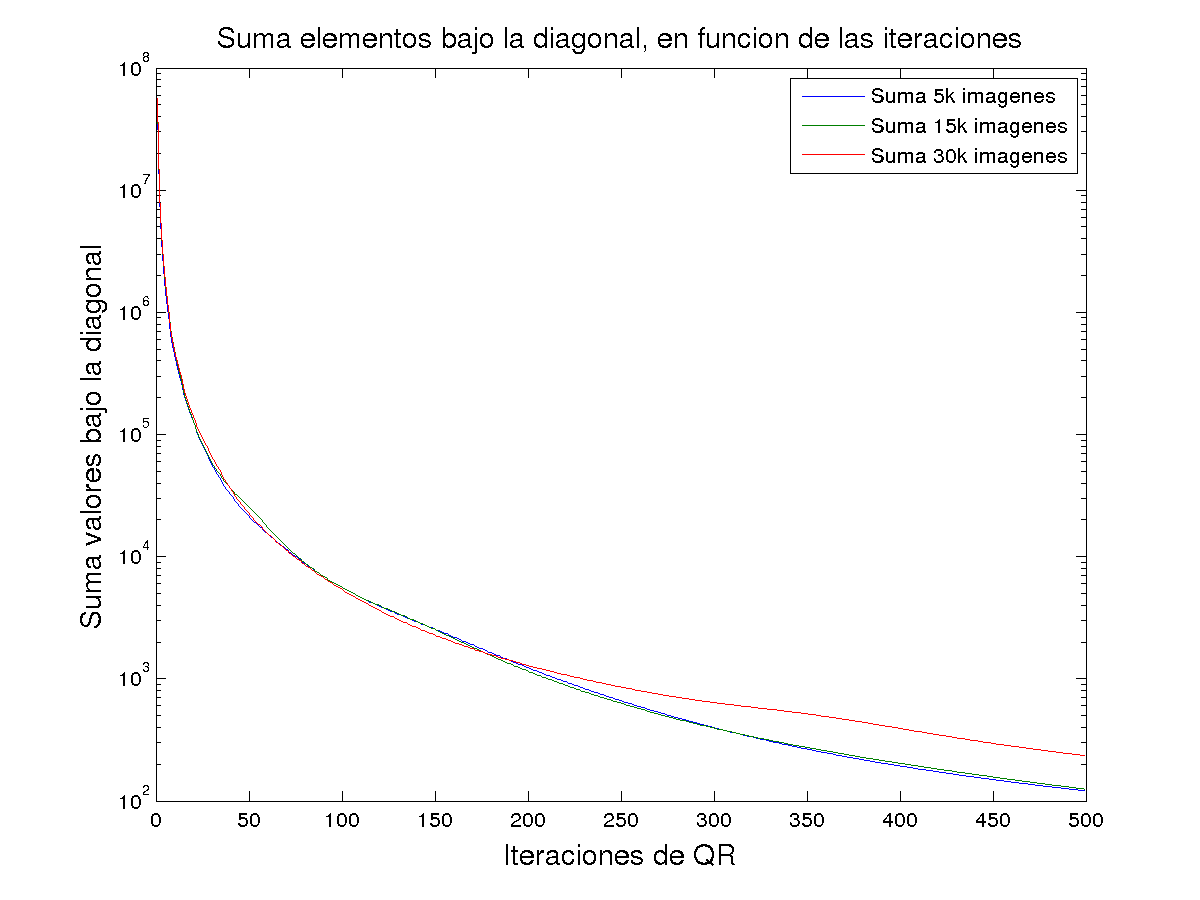
\includegraphics[width=\hrwidth]{plots/SUM.png}
\end {center}
\caption{Suma de los elementos bajo la diagonal para 5000, 15000 y 30000 im\'agenes
en funci\'on de la cantidad de iteraciones de QR.}
\label{fig:SUM}
\end{figure}

\begin{figure}[H]
\begin {center}
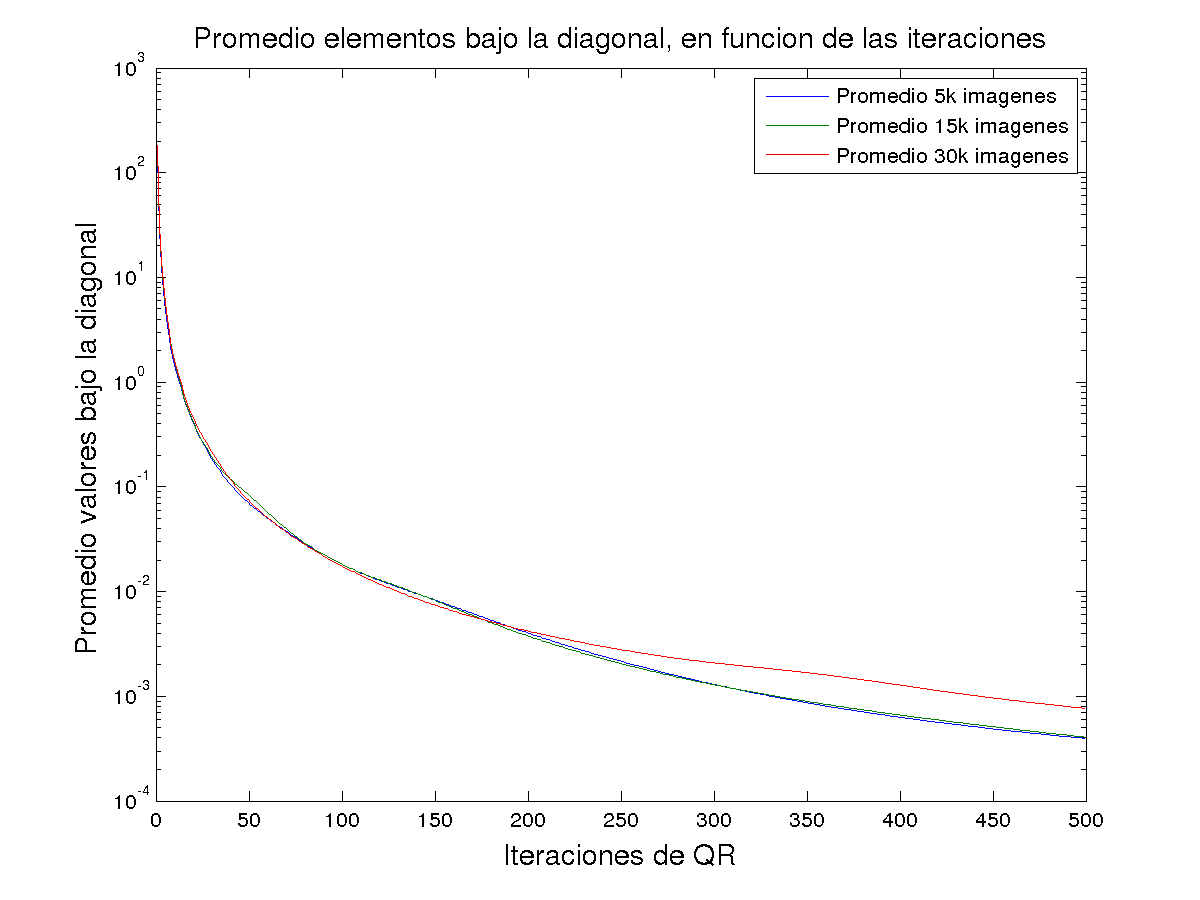
\includegraphics[width=\hrwidth]{plots/PROM.png}
\end {center}
\caption{Promedio de los elementos bajo la diagonal para 5000, 15000 y 30000 im\'agenes
en funci\'on de la cantidad de iteraciones de QR.}
\label{fig:PROM}
\end{figure}


\subsection{Promedio de Reconocimiento}
La m\'etodologia de implementaci\'on fue la siguiente: Se construy\'o una
m\'atriz de covarianza utilizando los primeros $n$ im\'agenes del dataset
\texttt{Training Data}. Luego, se tomaban $30000-n$ im\'agenes que se descartaban; para poder tomar 
siempre las mismas $t$ im\'agenes siguientes como im\'agenes de test, con sus 
correspondientes labels. A estos se les aplicaron las t\'ecnicas
de detecci\'on que hemos detallado antes y fuimos variando los $k$ componentes principales 
de las tuplas que tomabamos para hacer las cuentas de distancia.
Los gr\'aficos de HitRate est\'an hechos en funci\'on de $k$.
El Hitrate se define como el porcentaje de aciertos en la detecci\'on sobre el total de 
experimentos realizados. Decidimos expresarlo como fracci\'on de 1 (es decir,
Hitrate de $0.1$ equivale a $10\%$ de aciertos).

Tom\'amos siempre las mismas $t=500$ im\'agenes para todos los test, que representan
de manera proporcional a cada d\'igito.

Testeamos usando matrices de covarianza entrenadas con cantidad variable de im\'agenes.
\def \hrwidth {500pt}

\begin{figure}[H]
\begin {center}
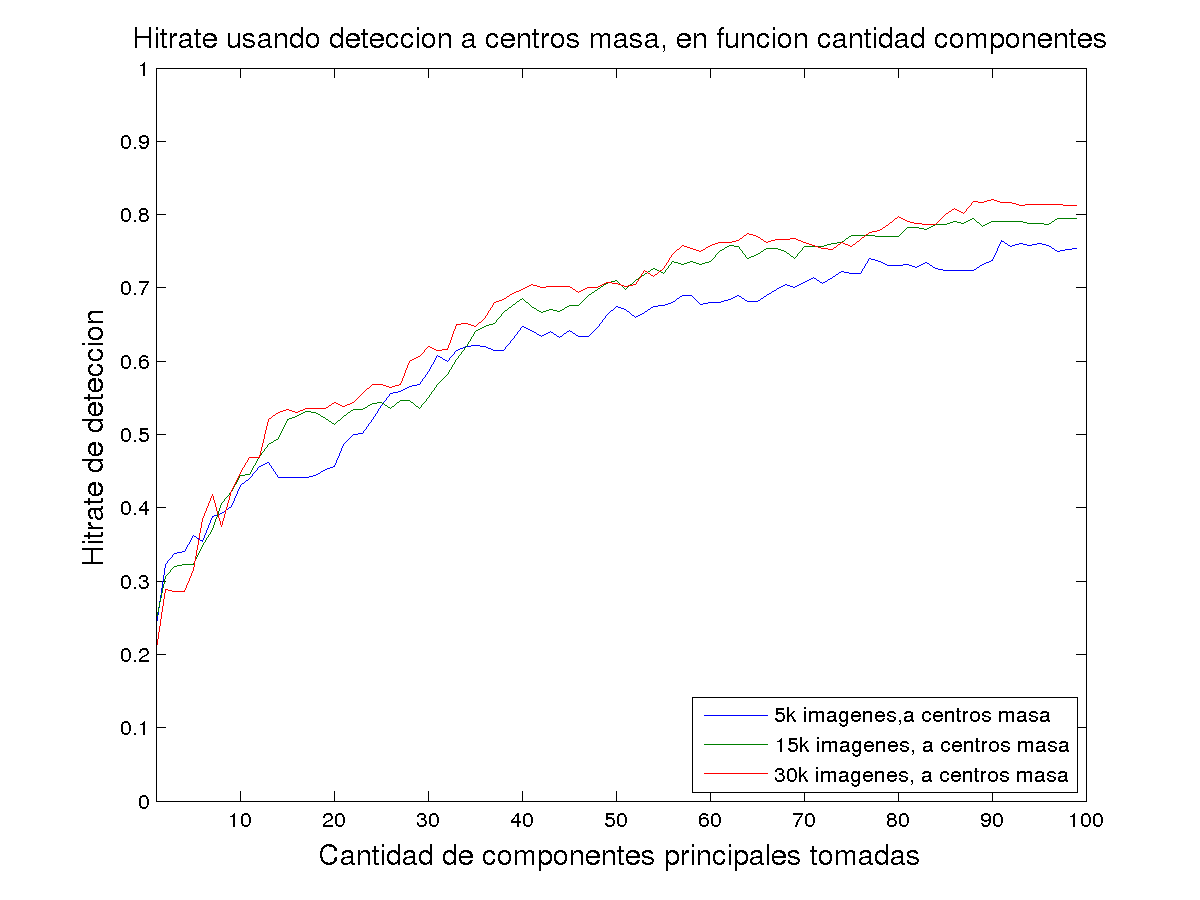
\includegraphics[width=\hrwidth]{plots/HR_N2.png}
\end {center}
\caption{Hitrate de detecci\'on de 500 im\'agenes utilizando la distancia a
centros de masa, entrenadas con distinta cantidad de ima\'genes}
\label{fig:HRN2}
\end{figure}

\begin{figure}[H]
\begin {center}
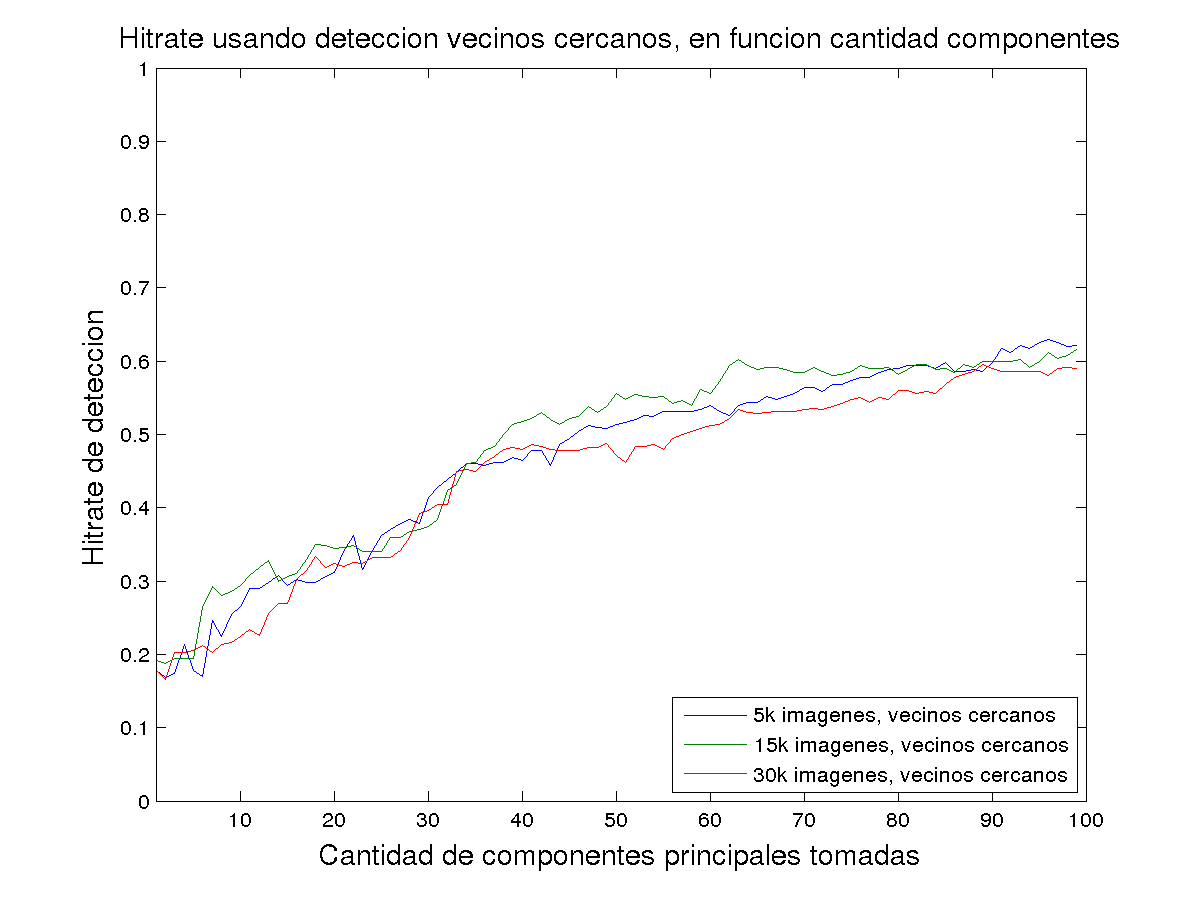
\includegraphics[width=\hrwidth]{plots/HR_VEC.png}
\end {center}
\caption{Hitrate de detecci\'on de 500 im\'agenes utilizando m\'etodo de
vecinos m\'as cercanos, entrenadas con distinta cantidad de ima\'genes}
\label{fig:HRVEC}
\end{figure}

%%%%%%%%%%%%%%%%%%%%%%%%%%%%%%%%%%%%%%%%%%%%%%%%%%%%%%%%%%%%%%%%

\subsection{Reconocimiento en funci\'on de iteraciones}
Dados los m\'etodos de detecci\'on, nos interesa ver como varia el hitrate
de acuerdo a la matriz generada con distinta cantidad de iteraciones de QR. En particular
utilizamos el m\'etodo de distancia a los promedios y 100 vecinos m\'as cercanos, todos
medidos usando norma 2.

\begin{figure}[H]
\begin {center}
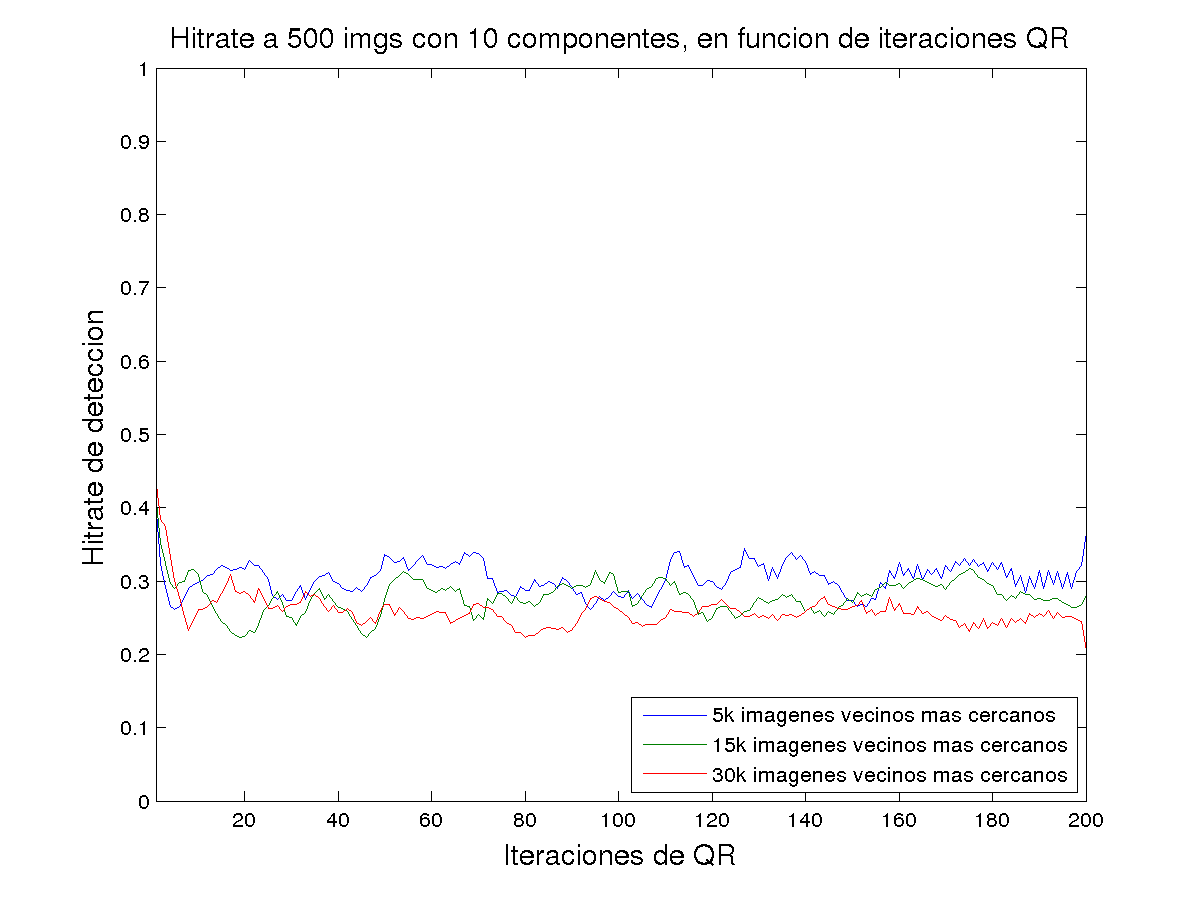
\includegraphics[width=\hrwidth]{plots/HR_10_1.png}
\end {center}
\caption{Hitrate en funci\'on de la cantidad de iteraciones en la generacion de la matriz
usando vecinos m\'as cercanos tomando 10 componentes principales}
\label{fig:HR10Neig}
\end{figure}


\begin{figure}[H]
\begin {center}
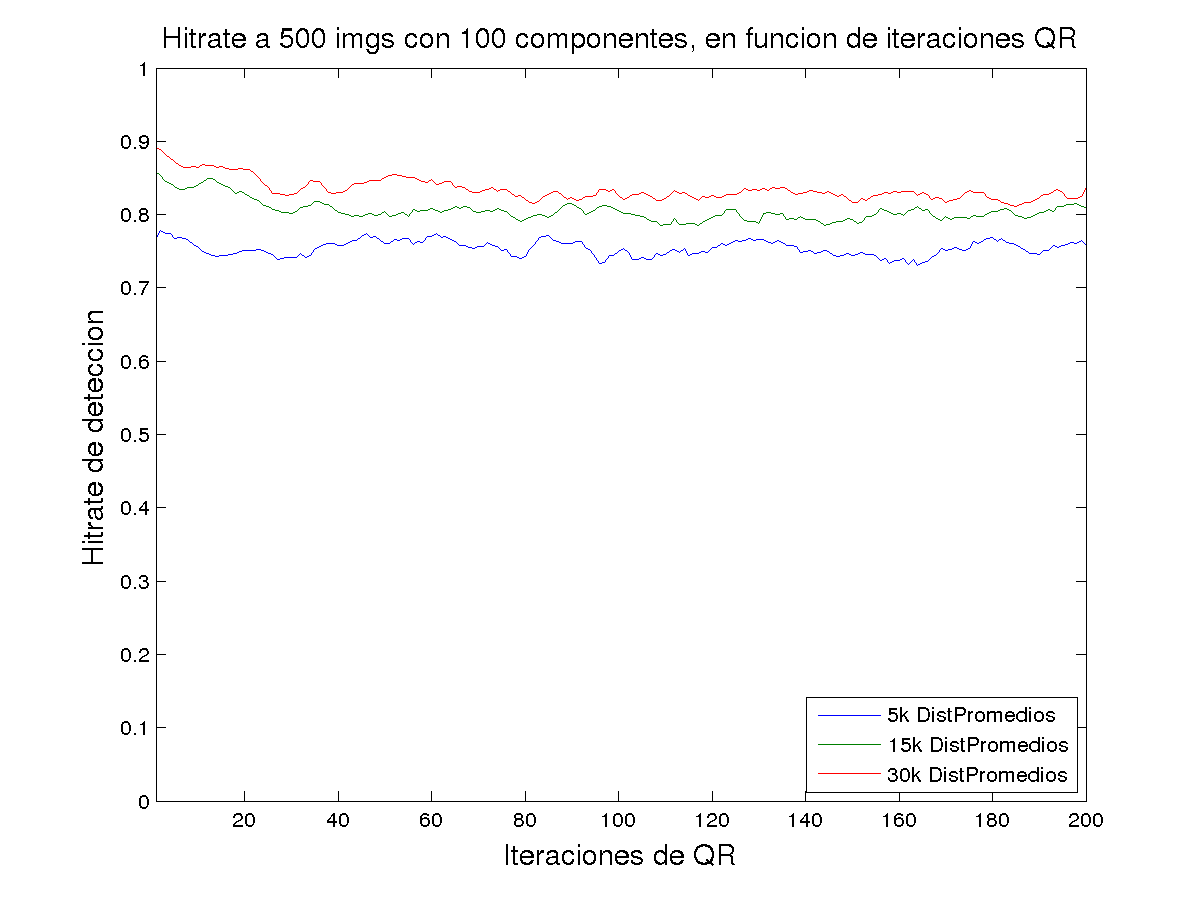
\includegraphics[width=\hrwidth]{plots/HR_100_1.png}
\end {center}
\caption{Hitrate en funci\'on de la cantidad de iteraciones en la generacion de la matriz
usando vecinos m\'as cercanos tomando 100 componentes principales}
\label{fig:HR10Neig}
\end{figure}


\begin{figure}[H]
\begin {center}
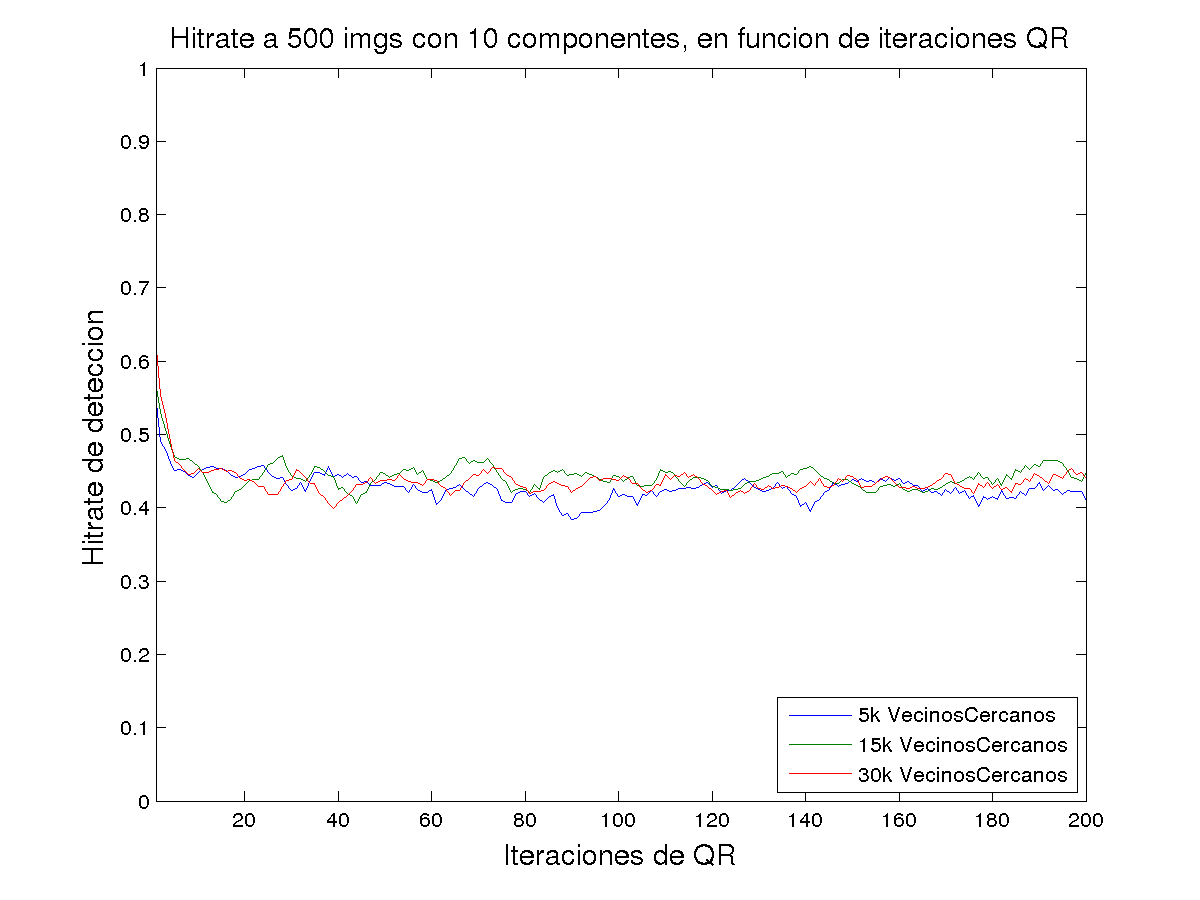
\includegraphics[width=\hrwidth]{plots/HR_10_0.png}
\end {center}
\caption{Hitrate en funci\'on de la cantidad de iteraciones en la generacion de la matriz
usando distancia a los promedios tomando 10 componentes principales}
\label{fig:HR10Avg}
\end{figure}


\begin{figure}[H]
\begin {center}
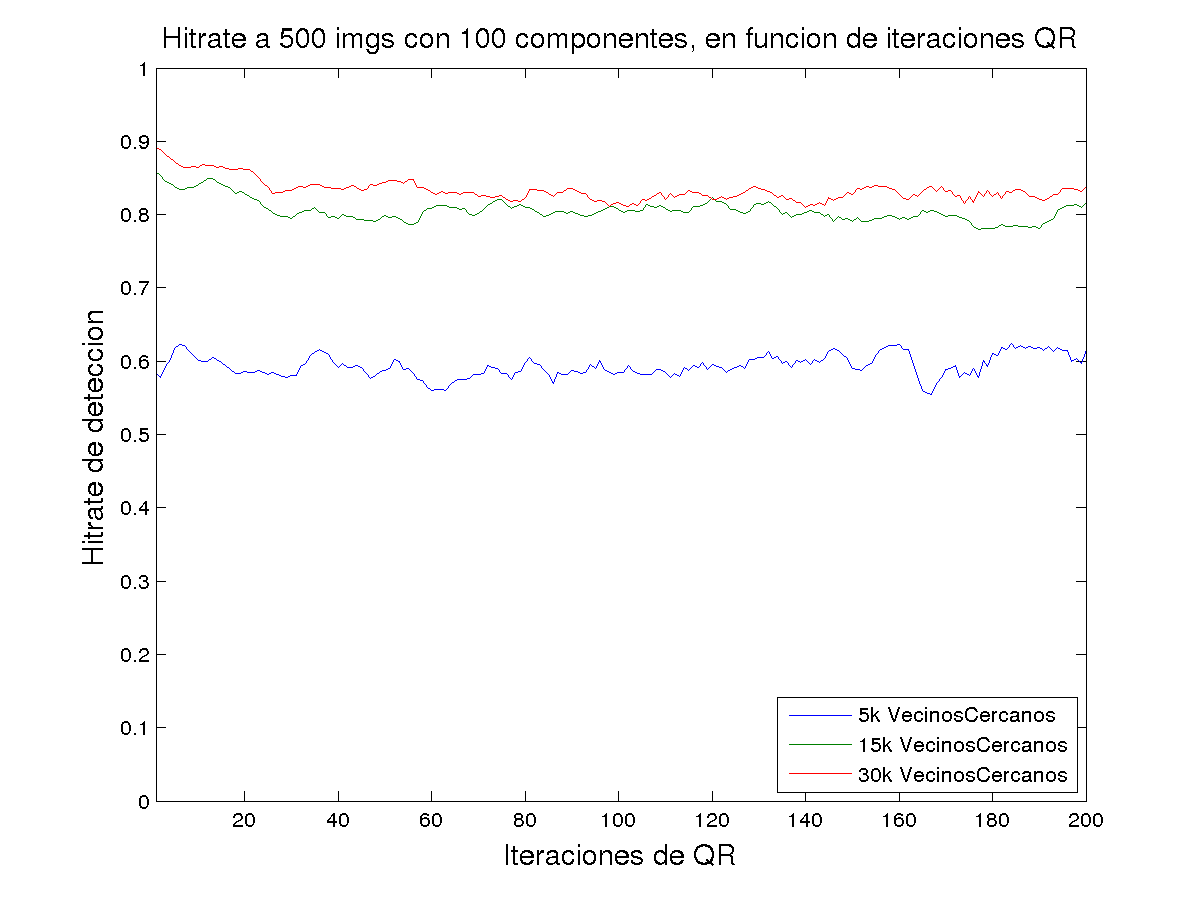
\includegraphics[width=\hrwidth]{plots/HR_100_0.png}
\end {center}
\caption{Hitrate en funci\'on de la cantidad de iteraciones en la generacion de la matriz
usando distancia a los promedios tomando 100 componentes principales}
\label{fig:HR100Avg}
\end{figure}








%%%%%%%%%%%%%%%%%%%%%%%%%%%%%%%%%%%%%%%%%%%%%%%%%%%%%%%%%%%%%%%%
\subsection{Reconocimiento por d\'igito}
Fijamos la matriz de covarianza entrenada con 30000 im\'agenes, ya que est\'a precalculada.
Siguiendo la misma metodolog\'ia, nos concentramos ahora en el HitRate individual
de cada d\'igito. Analizamos el HitRate de acuerdo a la metodolog\'ia de detecci\'on usada.

\def \pdwidth {500pt}

\begin{figure}[H]
\begin {center}
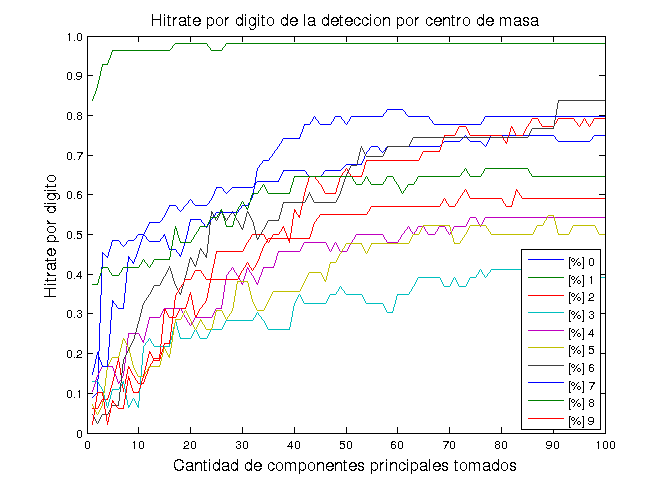
\includegraphics[width=\pdwidth]{plots/pordig-30kcv-norma2.png}
\end {center}
\caption{Hitrate por d\'igito de detecci\'on de 500 im\'agenes usando la matriz de covarianza entrenada con 30000 im\'agenes
clasificados por distancia a los promedios usando distancia a centro de masas}
\label{fig:HRD30kcv-n2}
\end{figure}

\begin{figure}[H]
\begin {center}
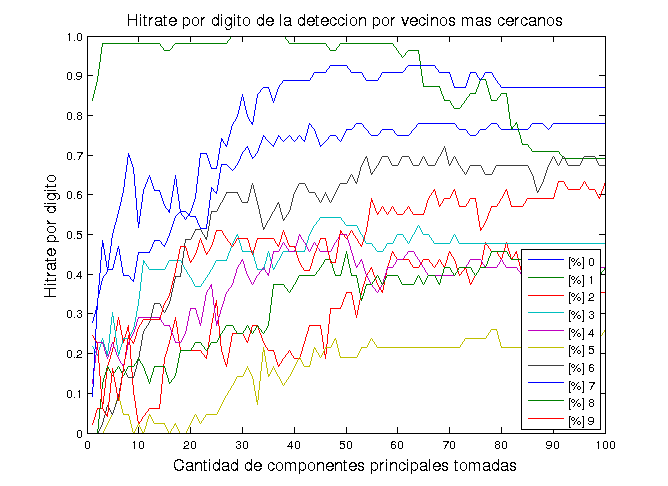
\includegraphics[width=\pdwidth]{plots/pordig-30kcv-top100.png}
\end {center}
\caption{Hitrate por d\'igito de detecci\'on de 500 im\'agenes usando la matriz de covarianza entrenada con 30000 im\'agenes
clasificados por distancia a vecinos m\'as cercanos}
\label{fig:HRD30kcv-dist100}
\end{figure}

\section{Heatmap de reconocimiento por d\'igito}
Ac\'a mostramos las equivocaciones y aciertos al reconocer cada d\'igito, variando la cantidad de componentes principales tomadas, hecho con la matriz de covarianza de
entrenada con 30000 im\'agenes y variando la cantidad de columnas tomadas. Eje X el valor detectado, eje Y el valor verdadero. El color marca la cantidad
de veces que se detect\'o un valor y a cual correspondia. Los valores negativo son solamente para que se grafiquen mejor,
son en realidad positivos.

\def \hmwidth {500pt}
\begin{figure}[H]
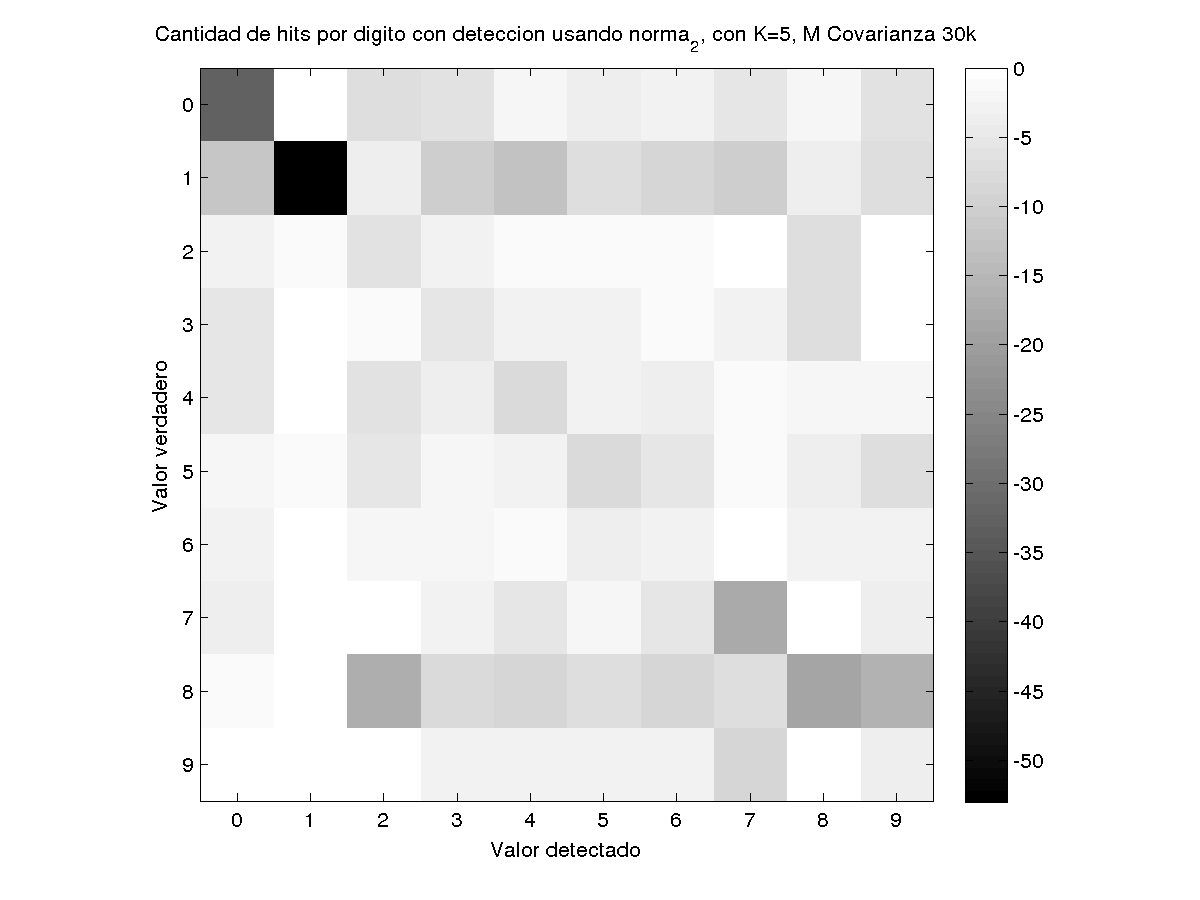
\includegraphics[width=\hmwidth]{plots/heatmap-30kcv-k5-norma_2.png}
\caption{Heatmap de aciertos por d\'igito de detecci\'on de 500 im\'agenes usando la matriz de covarianza entrenada con 30000 im\'agenes
clasificados por distancia a centros de masas tomando K=5}
\label{fig:HM30kcv-k5}
\end{figure}

\begin{figure}[H]
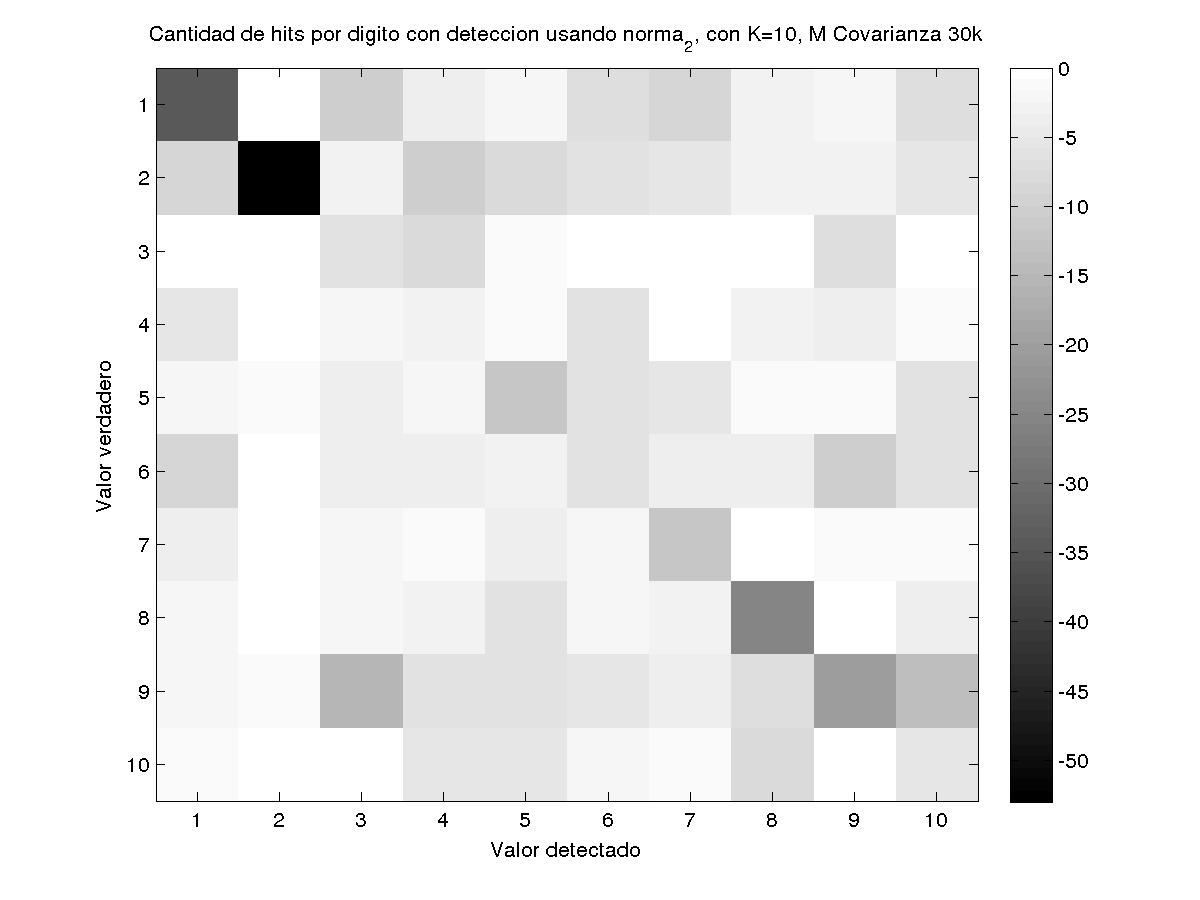
\includegraphics[width=\hmwidth]{plots/heatmap-30kcv-k10-norma_2.png}
\caption{Heatmap de aciertos por d\'igito de detecci\'on de 500 im\'agenes usando la matriz de covarianza entrenada con 30000 im\'agenes
clasificados por distancia a centros de masas tomando K=10 }
\label{fig:HM30kcv-k10}
\end{figure}

\begin{figure}[H]
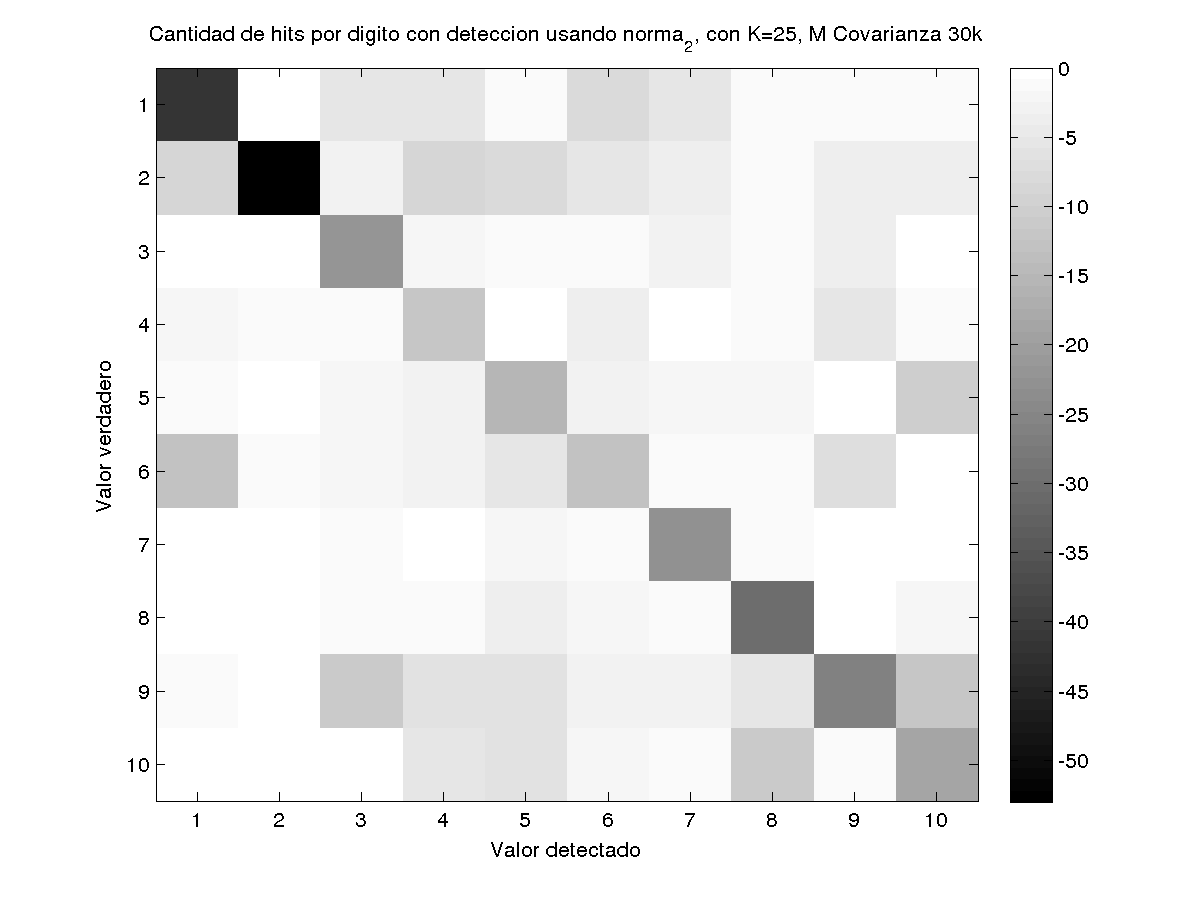
\includegraphics[width=\hmwidth]{plots/heatmap-30kcv-k25-norma_2.png}
\caption{Heatmap de aciertos por d\'igito de detecci\'on de 500 im\'agenes usando la matriz de covarianza entrenada con 30000 im\'agenes
clasificados por distancia a centros de masas tomando K=25 }
\label{fig:HM30kcv-k25}
\end{figure}

\begin{figure}[H]
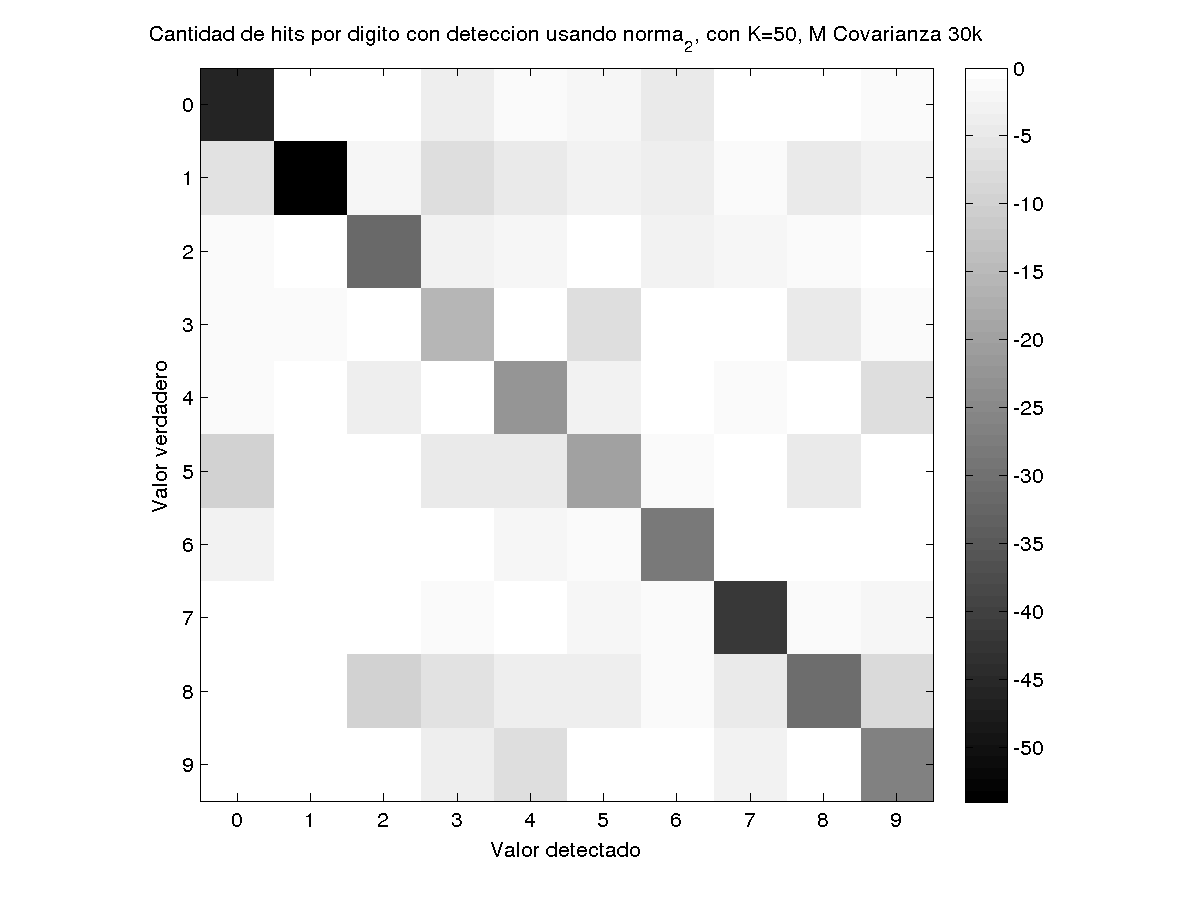
\includegraphics[width=\hmwidth]{plots/heatmap-30kcv-k50-norma_2.png}
\caption{Heatmap de aciertos por d\'igito de detecci\'on de 500 im\'agenes usando la matriz de covarianza entrenada con 30000 im\'agenes
clasificados por distancia a centros de masas tomando K=50 }
\label{fig:HM30kcv-k50}
\end{figure}

\begin{figure}[H]
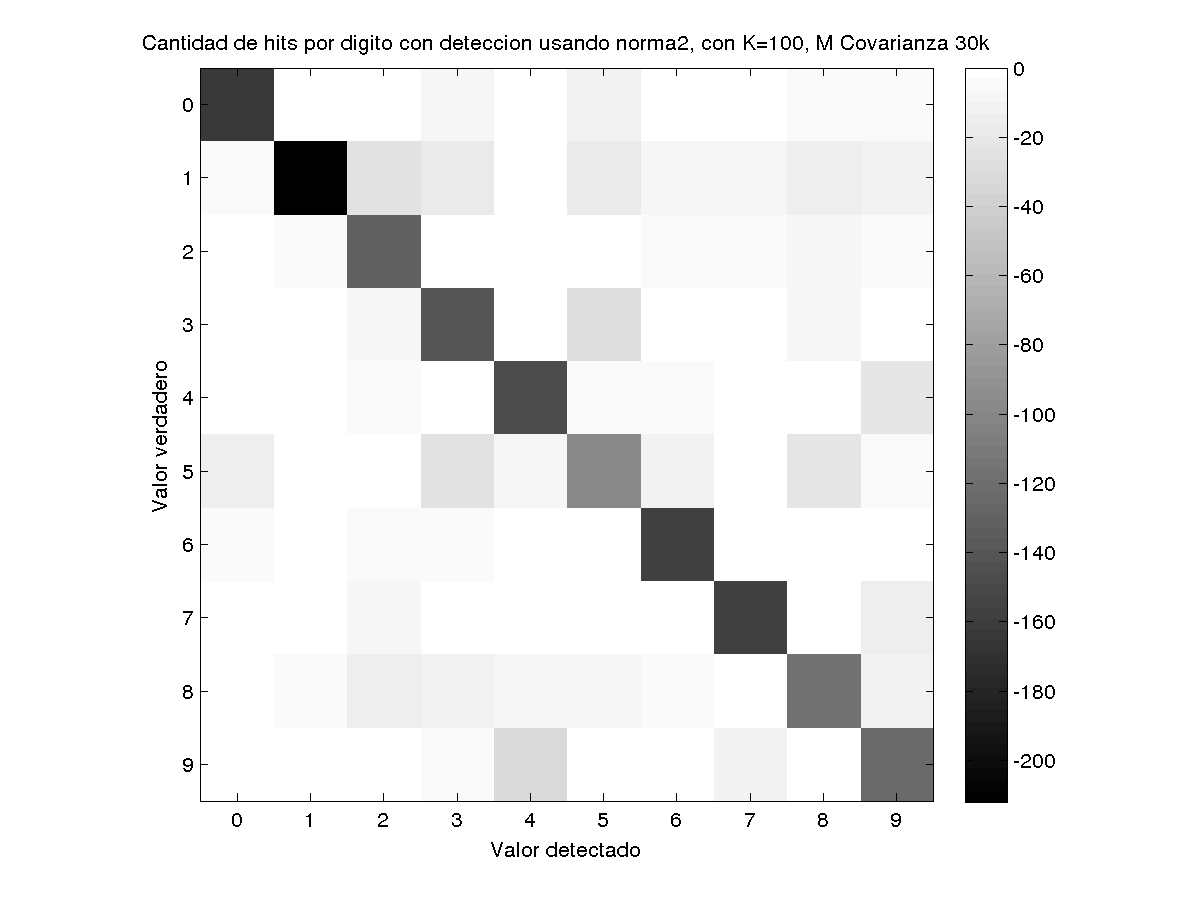
\includegraphics[width=\hmwidth]{plots/heatmap-30kcv-k100-norma_2.png}
\caption{Heatmap de aciertos por d\'igito de detecci\'on de 500 im\'agenes usando la matriz de covarianza entrenada con 30000 im\'agenes
clasificados por distancia a centros de masas tomando K=100 }
\label{fig:HM30kcv-k100}
\end{figure}
